%%% template.tex
%%%
%%% This LaTeX source document can be used as the basis for your technical
%%% paper or abstract. Intentionally stripped of annotation, the parameters
%%% and commands should be adjusted for your particular paper - title, 
%%% author, article DOI, etc.
%%% The accompanying ``template.annotated.tex'' provides copious annotation
%%% for the commands and parameters found in the source document. (The code
%%% is identical in ``template.tex'' and ``template.annotated.tex.'')

\documentclass[conference]{acmsiggraph}

\usepackage{authblk}

\TOGonlineid{45678}
\TOGvolume{0}
\TOGnumber{0}
\TOGarticleDOI{1111111.2222222}
\TOGprojectURL{}
\TOGvideoURL{}
\TOGdataURL{}
\TOGcodeURL{}



\title{A Greedy Heuristic using Redundancy for the Data Layout Problem}

\author[1]{Zachary DeStefano\thanks{zdestefa@uci.edu}}
\author[1]{Shan Jiang\thanks{sjiang1714@gmail.com}}
\author[1]{Gopi Meenakshisundaram\thanks{gopi.meenakshisundaram@gmail.com}}
\author[2]{Sung-Eui Yoon\thanks{toinsert}}
\pdfauthor{Zachary DeStefano,Shan Jiang,Gopi Meenakshisundaram,Sung-Eui Yoon}
\affil[1]{University of California, Irvine}
\affil[2]{KAIST}

\keywords{Data Layout Problem, Out-Of-Core Rendering, Cache Oblivious Mesh Layout}

\begin{document}

%% \teaser{
%%   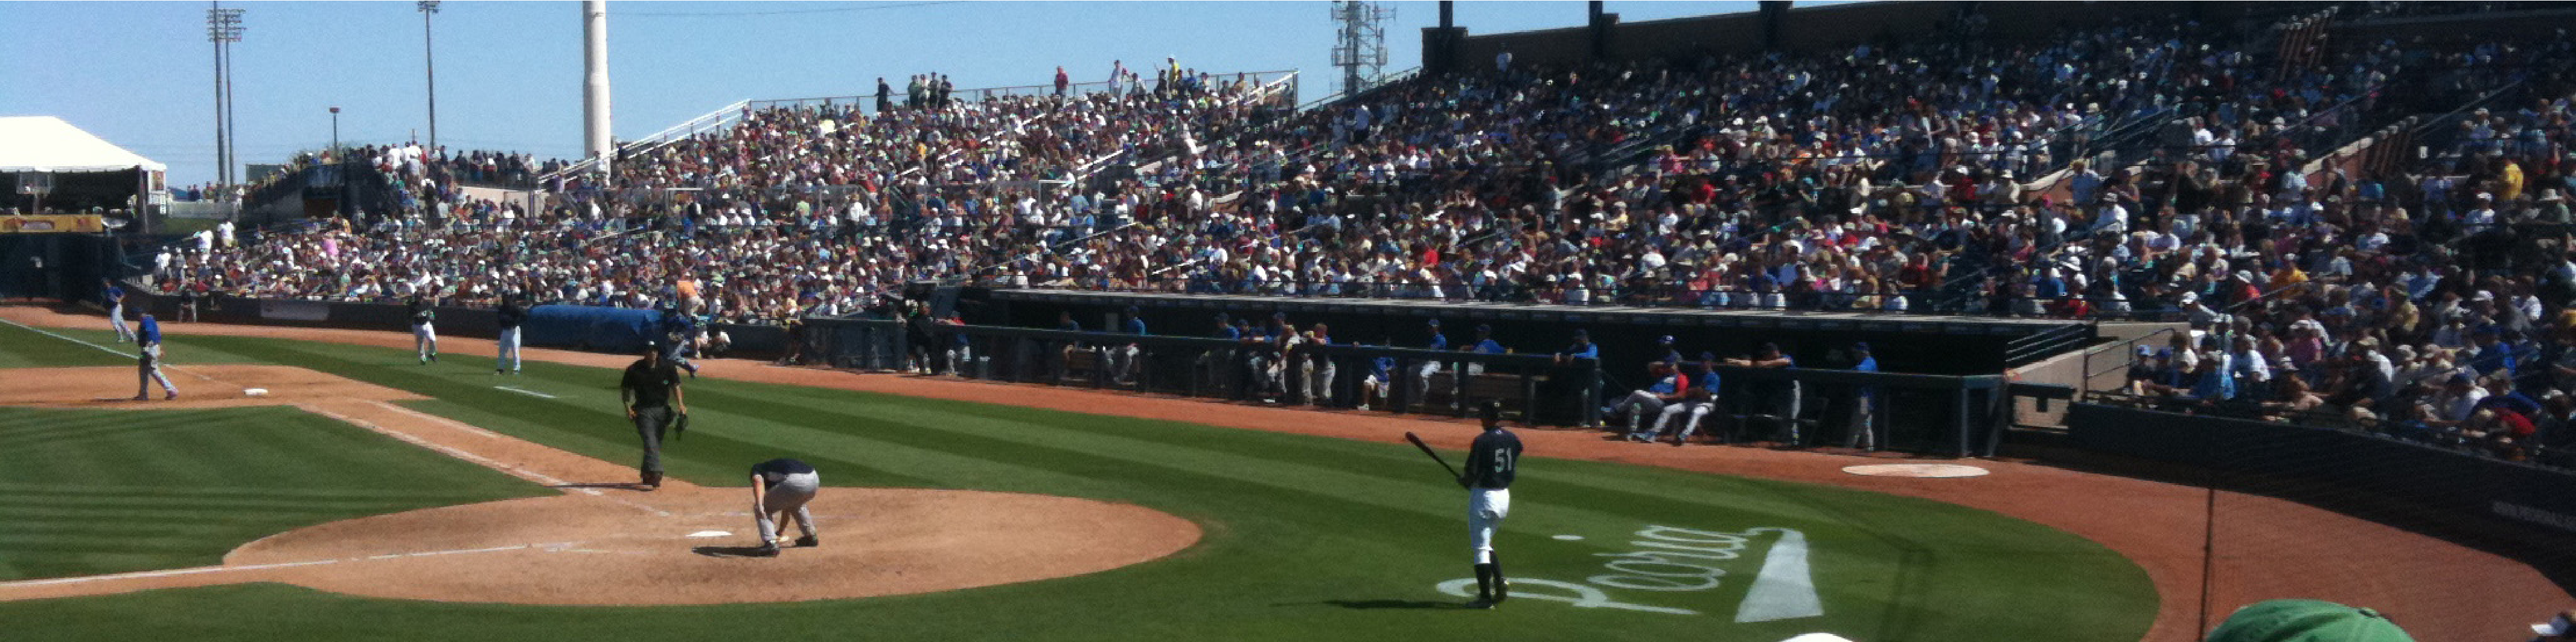
\includegraphics[height=1.5in]{images/sampleteaser}
%%   \caption{Spring Training 2009, Peoria, AZ.}
%% }

\maketitle

\begin{abstract}

In this paper, we present a greedy heuristic that uses redundancy to try and optimize seek time in a cache oblivious mesh layout. This is an important problem that appears when you are attempting to render massive amounts of geometric data that must be accessed together but cannot fit into main memory. We take previous work on optimizing the data layout and attempt to further reduce the seek time by inserting redundant data into key places. We have an algorithm that inserts redundant data units individually and ensures that each insertion is the one that reduces seek time the most at that step. In this way, we can minimize seek time using a limit on the amount of redundancy that we are allowed. This will prove to be an improvement over existing algorithms both analytically and experimentally. 

\end{abstract}

\begin{CRcatlist}
  \CRcat{I.3.6}{Computer Graphics}{Methodology and Techniques}{Graphics data structures and data types};
\end{CRcatlist}

\keywordlist

%% Use this only if you're preparing a technical paper to be published in the 
%% ACM 'Transactions on Graphics' journal.

\TOGlinkslist

%% Required for all content. 

\copyrightspace

\section{Introduction}

When attempting to render geometric models that contain hundreds of millions of vertices, the geometric data is too large to fit into main memory so only a small part of the model can be accessed at a given moment. When rendering a walkthrough application in this context, there is thus a seek time penalty that arises from getting data from the hard disk. This leads us to the Data Layout Problem, which is how do we lay out the data on the hard disk in such a way that minimizes the seek time required for the geometric data. Yoon et al \cite{cacheobliviouslayout} described this problem and came up with a metric to find the average seek time given the data layout as well as the access requirements of the data. An access requirement is a set of data units that will likely be accessed together during run-time.\\
\\
For the purposes of this paper, we are assuming that the relevant data units are laid out linearly on the disk. We are also assuming that the data units can be laid out in any order. Each data unit is assigned to one or more access requirements. With Yoon's definition, the average seek time ends up being the sum of the lengths of all the access requirements. We noticed that access requirements described in the paper can be very general and there could easily be data units that are far apart in the sequence but need to be accessed together. This led us to realize that if we copy data units and move them closer to other ones that share the same access requirement then we could save a lot of seek time without adding much storage space. \\
\\
We decided to formalize this idea in the form of a greedy algorithm that at each step copies the data unit which will improve seek time the most. Each step in the algorithm will copy a single data unit. We can thus stop the algorithm when we no longer have storage space to store more copies. This algorithm is thus a heuristic for the problem of given a certain amount of storage space that we are limited by, how can we minimize the seek time. 


\section{Related Work}

Massive model rendering has been a challenging field of research in computer graphics for decades. A large body of literature has been built on different aspects of solving this problem. Here we briefly discuss work in two main approaches in this topic, Out-Of-Core Rendering and Image-based Rendering. 

\subsection{Out-Of-Core Rendering}

Large-scale model rendering generally implies that the geometry data is so large that one must employ a secondary storage device during rendering. Thus, due to the nature of secondary storage devices and the architecture of modern computers, data fetching and data management for main memory can become performance bottlenecks during rendering. To remove or reduce these bottlenecks, research on out-of-core rendering aims at fetching, caching, and managing data in efficient ways. Coorea et al \cite{iwalk} introduced the iWalk system, in which octree-based spatialization is applied on geometry data, and this allowed only visible data to be retrieved from hard drives. Varadhan et al \cite{outofcore} also focused on isolating data required by each frame, but in a graph-based algorithm. A scene graph is generated in level of details and frame-to-frame visibility consistence. Parallel processing is also employed so that rendering the active part of the scene and fetching objects from the disk are done simultaneously. Sajadi et al \cite{pagebased} improved efficiency of out-of-core rendering by preprocessing the data set into a form of disk pages. The disk pages are self-contained data units with fixed size. This method avoids data management on the primitive level which reduces the time complexity by orders of magnitude. By utilizing a globally optimized data layout, caching can be further improved. Globally optimized data layout is an NP hard problem. Nevertheless, Yoon et al \cite{cacheobliviouslayout} provided a feasible method to try to compute it. Similar to other problems where an optimal permutation needs to be computed, they developed a hierarchical algorithm with a heuristic based on edge spans to get an approximated solution quickly.

\subsection{Image-Based Rendering}

Image-based rendering techniques reduce the geometry of a massive model to a view-independent mesh along with pre-rendered textures. The number of primitives to be rendered is much less than the original model. Therefore, both data transferring time and rendering time can be greatly saved. The major drawback of image-based rendering is the lack of geometry information. Zhang et al \cite{imagebasedrendering} presented a survey of image-based rendering techniques. These techniques involve sampling the space using a plenoptic function in the first stage and then rendering the continuous plenoptic function in the next stage. It is similar to the technique in signal processing of sampling a set of numbers and then using those samples to get the continuous function and reconstructing the continuous function. The paper goes into detail on various applications of these techniques. Li et al \cite{compressionimagebased} explored various compression methods for image-based rendering. Specifically, they explored the benefits of three compression algorithms. All three proved to be able to achieve real time rendering of large models and they vary in the complexity of the decoding and the compression ratio they are able to achieve. 

\subsection{Seek Time and Redundancy-based solutions}

In real time rendering, time spent on one frame can be roughly divided into data fetching time, online processing time, and rendering time. Data fetching time can be further decomposed into seek time and data transfer time. Sajadi et al \cite{ssdpaper} explored the reasons for the performance advantage of Solid-State Drives (SSD) over Hard-Disk Drives (HDD). The result shows clearly constant seek time of SSDs is the major reason that fetching data on SSDs is generally faster and more consistent than HDDs. Jiang et al \cite{singleseeklayout} minimized disk seeks to one or less for each frame by storing multiple copies of same data at different locations of secondary storage devices. These extra copies will be referred to as redundancy. The paper successfully showed that limited seeks lead to improvement of performance. However, to keep number of seeks being one or less, a large amount of redundancy is necessary, which is not practical for many applications. Jiang et al \cite{optimizingredundancy} generalized this approach by relaxing the number of seeks to a small threshold. This threshold is determined by time budget of each frame. In this way, the number of seeks required is relaxed to minimize amount of redundancy. This optimization is done through integer linear programming. This approach ended up reducing the amount of redundancy significantly. The algorithm however does not take data layout into account and is thus not an optimal solution.

\section{Greedy Redundancy-based Cache Oblivious Mesh Layout Algorithm}

We can formulate this problem in the following way given Yoon's metric. We are given a linear sequence of data units as well as one or more access requirements that each data unit is assigned. In Yoon's paper, he is only allowed to move the data units around. In this paper, we are allowed to copy data units, move them, and delete old copies of data units. Given this input and these 3 operations, we need to figure out how to minimize the sum of the lengths of the access requirements using the least amount of extra space as possible. For this paper, we assume that we are given a certain amount of space and need to figure out how much we can minimize the seek time.\\
\\
The algorithm in Yoon et al. computes a locally optimal solution without considering copying data units. Our algorithm takes over afterwards. W take a data unit and copy it to a place that will mean shortening at least one of the access requirements that is attached to it. If the new data unit shortens all the access requirements attached to it, then we delete the old data unit. \\
\\
There are important issues to consider in order to make this idea into an algorithm. First of all, we need to know which data units in each access requirement we should consider. We then need to figure out which access requirements to take care of first. We need to know where to insert the copied data unit. Once we copy a data unit and find its location, we need to consider whether its other access requirements should use the old or new copy. Finally, we need to decide when to stop the algorithm.  

\subsection{Which data unit in each access requirement}

Since we only care about the length of each access requirement and we can only copy a single data unit at one time, we will only be copying the data units that are on the endpoints of an access requirement. This will greatly reduce the search space of data units to consider for copying. \\
\\
The figure below shows an example access requirement. As can be observed, if we move any of the interior units, the access requirement will stay the same length or become larger. However if we move the start or end unit, the access requirement will become shorter. 
\begin{figure}[ht]
\centering
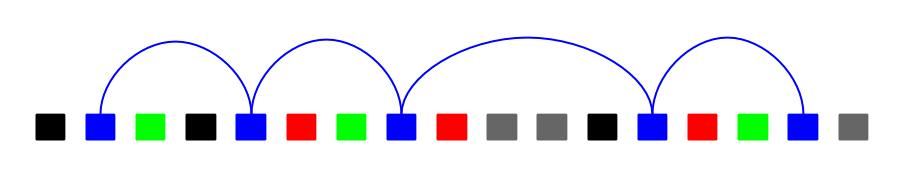
\includegraphics[width=3in]{SingleAR_start.jpg}
\caption{Data Units for a single access requirement}
\end{figure}

\subsection{Where to locate data unit}

Since we are only allowed to move one data unit at a time, in order to maximize our benefit to our current access requirement, we want to copy the start data unit to somewhere between the one after the first one and the last one. In the same manner, if the end data unit is better, we want to copy it to somewhere between the first one and the one before the last one. Below is the access requirement from the above figure with an arrow showing the locations where the start unit can be moved to. \\
\begin{figure}[ht]
\centering
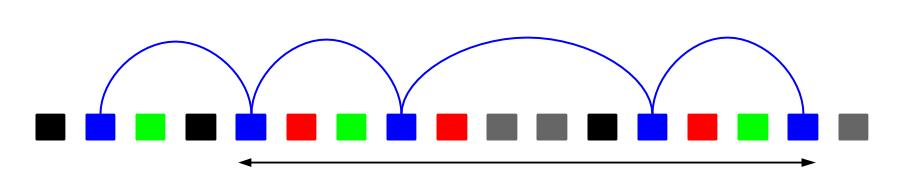
\includegraphics[width=3in]{SingleAR_afterCopy1.jpg}
\caption{Interval where the start data unit can be copied to}
\end{figure}
\\
By doing this we are guaranteed to reduce the seek time for the access requirement we care about. For our own access requirement, it won't matter where in that interval we place our data unit. However, for the other access requirements that overlap a potential place to insert our data unit, we are adding one unit of seek time. Therefore, we want to find which place will interrupt the least number of access requirements. We can assume that we have already precomputed the number of overlaps at each unit. We now have the problem of given a sequence of numbers and an arbitrary block of that sequence, what is the least number in that block. For our purposes, we will do a linear search through each entry in the block in order to find the ideal entry. While in theory there are more efficient solutions, they will be impractical for our purposes, as we will describe in the next section.

\subsection{Which data unit is used by each access requirement}

A given data unit will have a few access requirements attached to it. Thus when it is copied, it may benefit other access requirements besides the one you are currently working on. For the other access requirements, if they are shorter by using the new copy then they should do that. Otherwise, they should stick to the old copy.

\subsection{Which overall data units should be copied}

We now have established a mechanism for shortening access requirements by copying data and potentially being able to delete the old copy. We now need to figure out how to use this information to decide in what order the copying should be done. For each data unit, its total benefit is the amount that is reduces the total seek time ($EST$), which is the sum of the lengths of the access requirements. \\
\\
For a given data unit to be copied to a specified location, let $k_i$ be the benefit to access requirement $i$ that is attached to the data unit. We will say that $k_i=0$ if the access requirement will use the old copy and $k_i>0$ if the access requirement will use the new copy. Let $I$ be the set of access requirements attached to the data unit. Finally, let $M$ be the number of overlapping access requirements at the location chosen. We can now describe the benefit as follows:
\[
\Delta EST = M - \sum_{i \in I} k_i
\]
Before doing any actual copying, we will compute the above described benefit for each start and end data unit for each access requirement. We will put all the benefits into a binary search tree sorted in ascending order by benefit amount. That way we will easily be able to choose the data unit that provides the most negative change in expected seek time. We will also make a special list $L$ of cases where a data unit is copied then deleted because all the access requirements will benefit. \\
\\
Because doing the copying in $L$ does not increase the storage, we will first go through that list and do the copying. Once that list is empty we will take the data unit in the binary search tree that provides the most benefit and perform the copy. We will then recompute $L$ and the binary search tree. We will continue to do those steps until we have run out of available space for redundancy.  

\section{Run-time and Storage Analysis}

We now need to analyze the running time and storage requirements of our algorithm. We will denote $N$ as the number of data units and $A$ as the number of access requirements. We will use $k$ as the average length of a single access requirement. The variable $Q$ will represent the number of runs of the redundancy and new copy loop. The average number of overlapping access requirements is proportional to the number of data units multiplied by the redundancy factor $r$, which is the amount of redundancy if we have a single-seek layout. Therefore, the number of overlapping access requirements is O(rN). \\
\\
The Initial Construction loop is run on all A access requirements. It involves finding all the benefit information and putting it into a heap so that it is easy to figure out the best access requirement to modify first. There are log(A) operations to insert the data into the heap and a constant number of operations plus O(k) operations for the search of the AR to get the benefit information. Thus it takes a total of $O(A \cdot k \cdot logA)$ operations to do the initial construction. \\
\\
With the new copy and redundancy loops, there are O(rN) overlapping access requirements and a constant number of operations for each access requirement. Then, the algorithm reforms the heap and updates the nodes in the AR. With that, there are $O(log(A))$ operations done a constant number of times plus O(k) operations for updating the data nodes in the access requirement. Thus the redundancy and new copy loop takes $O(Q(k \cdot logA + rN))$ operations. \\
\\
This means that in total, our algorithm takes $O( k \cdot logA (Q+A) + rN)$ operations. 

\subsection{Linear search justification}

Here I justify why we do a simple linear search in the part of the algorithm where we decide where to put the new data unit. The original problem is to find the least number in an arbitrary block of a list. If $k$ is the size of the access requirement, then this gives us $O(k)$ query time. Updates will also be $O(k)$ and construction will be $O(N)$ with N being the number of data units. There are other approaches, such as a range tree or dynamic programming, that may produce better query times, but their construction and update times will be worse as well as their storage. \\
\\
With dynamic programming, we would have to maintain a matrix where an entry $(i,j)$ would contain the minimum value in that range. This would give us a $O(1)$ query time but the construction and storage would be $O(N^2)$ where N is the number of data units. The update time would be $O(N)$ when we add a data unit. Since the $N$ for this problem domain is in the hundreds of millions, that is an unacceptable storage bound. The construction run time would also be prohibitive given the magnitude of our input. \\
\\
We could use a range tree. The initial binary search tree would be sorted by index and at each entry would be a pointer to a binary search tree sorted by value. If we put the min value at each of the nodes of the initial tree, we can speed up our queries. We would get a $O(log N)$ query time, but our construction time and storage would be $O(N log N)$. Updating the data structure would take at a minimum $O(k log(N))$ time if we do careful indexing and only update the nodes that need to be updated. If we have a large access requirement, then this would represent a significant improvement in query time however given our exceptionally large input, the construction, storage, and update bounds are too prohibitive.  


\section{Theoretical Improvements over existing algorithms}

The first part of the algorithm will produce a better solution than proposed by Yoon without adding extra units. This is because our algorithm will consider cases where data units are close to each other but in different blocks of units that would be arranged in Yoon's algorithm. Consider a case where we have two access requirements of 5 data units each. If they are spread across the sequence, then Yoon's algorithm would not consider grouping them together, since they would be in different blocks of 5. **INSERT PICTURE OF THIS AND MORE DETAIL** \\
\\
Existing algorithms do not consider redundancy. Even if we find a polynomial solution to the data layout problem, we can actually achieve a seek time better than the optimal one without redundancy. Figure 1 shows a case where that happens. The total seek time is 11 units. Without redundancy, the optimal solution is shown in Figure 2. The seek time has been reduced to 9 units. With redundancy, the total seek time is now the minimum required which is 7 units, as shown in Figure 3. While a reduction from 9 to 7 units may not seem dramatic, when this result is scaled up to the hundreds of millions, this makes a big difference in seek time, which we saw in practice.\\

\begin{figure}[ht]
\centering
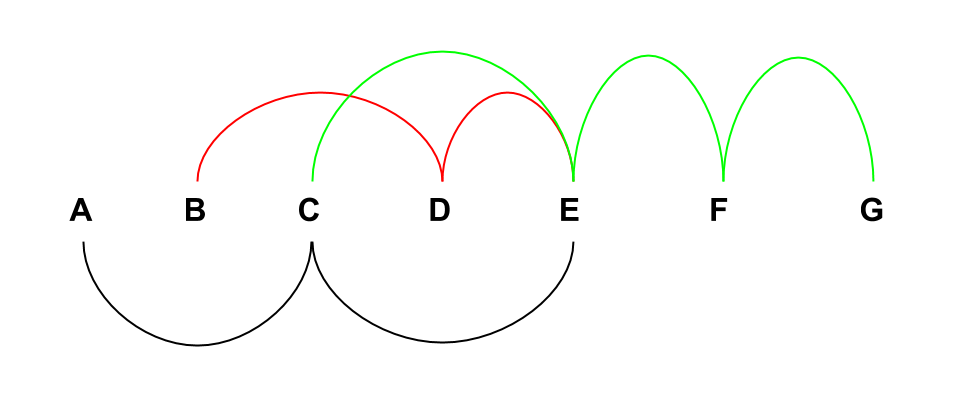
\includegraphics[width=3in]{examplePic_startingProblem.png}
\caption{Data Units with varying access requirements}
\end{figure}

\begin{figure}[ht]
\centering
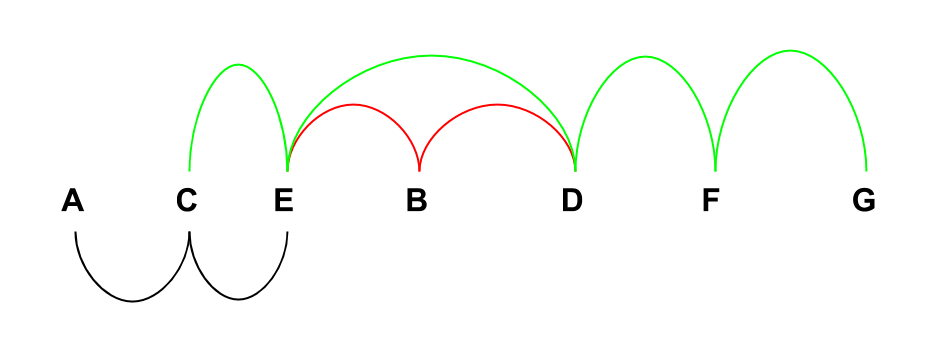
\includegraphics[width=3in]{examplePic_woRedundancy.png}
\caption{Optimal layout without redundancy}
\end{figure}

\begin{figure}[ht]
\centering
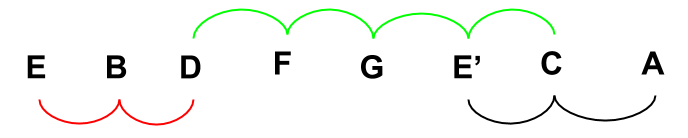
\includegraphics[width=3in]{examplePic_withRedundancy.png}
\caption{Optimal layout with redundancy}
\end{figure} 

\section{Experimental Results}

**INSERT THE INFO FROM SHAN'S THESIS**


\section{Conclusion and Future Work}

We have shown that we have a quadratic time algorithm with quadratic storage space for the Data Layout Problem. It achieves significant results analytically and experimentally. When walking through an extremely detailed 3D model, this algorithm can be used to ensure that the performance will not suffer. If we give the algorithm the proper access requirements with this 3D model, then the performance will be even better.\\
\\
This leads to a logical extension of this work. Since we have a good algorithm that takes over once we know the access requirements, we should figure out how to ensure there are good access requirements to begin with. One idea on how to ensure this is to check the usage history of an application and group data units together if they are accessed together with high probability. This could even be done dynamically in the sense that after a certain amount of usage and repeating on a regular basis, you recompute the optimal access requirements and then use that to recompute the optimal layout. 

\section{Acknowledgements}

To Robert, for all the bagels.

\bibliographystyle{acmsiggraph}
\bibliography{finalPaperRefs}

\section{Appendix}

\subsection{Algorithm Summary}

\begin{verbatim}

Initialize AR heap and newCopy list
for each accessRequirement P's head node and tail node U:
     Set benefit to distance from U to next or previous node
     Let destination be spot with least number of overlapping access requirements
     For each access requirement T that also uses U
          See if T will be shorter by using new copy. Add T to oldCopyList if not.
          Add that to benefit if so
     Add benefit to heap
     If oldCopyList is empty then add U to newCopy list
while newCopy is not empty:
     take out random element and move the node
     Update AR heap and newCopy list
while there exists more space for redundancy:
     pop best element from heap
     copy the element U to its destination
     update affected access requirements
     update heap

\end{verbatim}

\end{document}
